\documentclass[oneside,senior,etd]{BYUPhys}

\usepackage{cmap} % Для корректной кодировки в pdf
\usepackage[utf8]{inputenc}
\usepackage{rotating}

\usepackage[russian]{babel}
\usepackage{amsfonts} % Пакеты для математических символов и теорем
\usepackage{amstext}
\usepackage{amssymb}
\usepackage{amsthm}
\usepackage{graphicx} % Пакеты для вставки графики
%\usepackage{subfig}
\usepackage{color}
\usepackage[unicode]{hyperref}
\usepackage[nottoc]{tocbibind} % Для того, чтобы список литературы отображался в оглавлении
\usepackage{verbatim} % Для вставок заранее подготовленного текста в режиме as-is
\usepackage{listings}

\newcommand{\sectionbreak}{\clearpage} % Раздел с новой станицы

\usepackage{tikz}
\usepackage{pgfplots}
\usetikzlibrary{arrows,positioning}
\usepackage{adjustbox}

\usepackage{makecell}
\usepackage{booktabs}
\usepackage{boldline}

\usepackage{xcolor}
\usepackage{soul}
\usepackage{url}
\usepackage{multirow}
\usepackage{amsmath}

\usepackage{pifont}
\usepackage{indentfirst} % Делать отступ в начале первого параграфа

\usepackage{minted}

\usepackage[inline]{enumitem}
\usepackage{subcaption}

\usepackage[russian]{cleveref}

\renewcommand
\listingscaption{Листинг}

% Общие параметры листингов
\lstset{
  %frame=TB,
  showstringspaces=false,
  tabsize=4,
  basicstyle=\linespread{1.0}\tt\small, % делаем листинги компактнее
  breaklines=true,
  texcl=true, % русские буквы в комментах
  captionpos=b,
  aboveskip=\baselineskip,
  commentstyle=\tt
}

\newcommand{\todo}[1]{\textcolor{red}{#1}}

% DEBUG
% \usepackage{showframe}

\Faculty{Факультет вычислительной математики и кибернетики}
\Chair{Кафедра системного программирования}
\Course{Суперкомпьютерное моделирование и технологии}
\Year{2025}
  \Date{23 Октября}
  \City{Москва}
  \AuthorText{Автор:}
  \Author{Егоров Илья Георгиевич}
  \AuthorEng{Ilya Yegorov}
  \AcadGroup{627}

  \TitleTop{Многопоточная реализация с использованием OpenMP}
  \TitleMiddle{решения гиперболического уравнения в частных производных}
  % Раскомментируйте, если нужны еще строчки названия
  \TitleBottom{на трехмерном прямоугольном параллелепипеде}
  % Uncomment if you need English title
  % \TitleTopEng{Thesis theme, first line}
  % \TitleMiddleEng{Thesis theme, second line}
  % \TitleBottomEng{Thesis theme, third line}

\docname{ОТЧЁТ}                                      

%%%% DON'T change this. It is here because .sty does not support cyrillic cp properly %%%%
\TitlePageText{Титульная страница}
\University{Московский государственный университет имени М.В.Ломоносова}
\GrText{группа}
\ListingText{Листинг}
\AlgorithmText{Алгоритм}

% Set PDF title and author
\hypersetup{
  pdftitle={\PDFTitle},
  pdfauthor={\PDFAuthor}
}

\begin{document}
\fixmargins
 \makepreliminarypages

\oneandhalfspace

\pdfbookmark[section]{\contentsname}{toc}
\tableofcontents

\section{Описание задания и программной реализации}

\subsection{Постановка задачи}

В трёхмерной замкнутой области $\Omega = [0, L_x] \times [0, L_y] \times [0, L_z]$
для $t \in [0, T]$ требуется найти решение $u(x,y,z,t)$ задачи
\begin{equation}
\begin{cases}
  u_{tt}(x,y,z,t) = a^2\Delta u(x,y,z,t)    \\
  u(x,y,z,0) = \phi(x,y,z)                  \\
  u_t(x,y,z,0) = 0                          \\
  u(0,y,z,t) = u(L_x,y,z,t) = 0             \\
  u(x,0,z,t) = u(x,L_y,z,t)                 \\
  u(x,y,0,t) = u(x,y,L_z,t) = 0
\end{cases}
\end{equation}

гдe $u(x,y,z,t) = sin\frac{\pi x}{L_x} sin\frac{2\pi y}{L_y} sin\frac{3\pi z}{L_z}
cos(a_t t)$, $a_t = \frac{\pi}{2}\sqrt{\frac{1}{L_x} + \frac{4}{L_y} +
\frac{9}{L_z}}$~--- точное аналитическое решение, $\phi(x,y,z) = u(x,y,z,0) =
sin\frac{\pi x}{L_x} sin\frac{2\pi y}{L_y} sin\frac{3\pi z}{L_z}$
и $a^2 = \frac{1}{4}$.

\subsection{Численный метод решения задачи}
Пусть заданы $N, K \in \mathbb{N}$, тогда пусть $h_x = \frac{L_x}{N}$,
$h_y = \frac{L_y}{N}$, $h_z = \frac{L_z}{N}$, $\tau = \frac{T}{K}$ и
$\omega_{h\tau} = \overline{\omega_h} \times \omega_{\tau}$, где \\
$\overline{\omega_h} = \{(x_i, y_j, z_k) | x_i = ih_x, y_j = jh_y, z_k = kh_z,
i,j,k \in \overline{0, N} \}$ \\
$\omega_{\tau} = \{t = n\tau, n \in \overline{0, K}\}$

Пусть $\omega_h = int \overline{\omega_h}$, т.е. внутренние узлы сетки. \\
Пусть $u_{ijk}^n = u(x_i, y_j, z_k, t_n), \phi_{ijk} = \phi(x_i, y_j, z_k)$

Тогда
\begin{align*}
  & u_{0jk}^n = u_{Njk}^n = u_{ij0}^n = u_{ijN}^n = 0,
    & i,j,k \in \overline{0, N}, n \in \overline{0, K} \\
  & u_{i0k}^n = u_{iNk}^n, u_{i1k}^n = u_{iN + 1k}^n,
    & i,k \in \overline{0, N}, n \in \overline{0, K} \\
  & u_{ijk}^0 = \phi_{ijk} = \phi_{ijk} = \phi(x_i, y_j, z_k),
    & (x_i, y_j, z_k) \in \omega_h \\
  & u_{ijk}^1 = u_{ijk}^0 + \frac{a^2\tau^2}{2}\Delta_h \phi_{ijk}
    & (x_i, y_j, z_k) \in \omega_h \\
  & u_{ijk}^{n + 1} = 2u_{ijk}^n - u_{ijk}^{n - 1} + \Delta_h u_{ijk}^n
    & (x_i, y_j, z_k) \in \omega_h
\end{align*}

Здесь $\Delta_h$~--- семиточечный разностный аналог оператора Лапласа: \\
\begin{align*}
\Delta_h u_{ijk}^n = \frac{u_{i + 1jk}^n - 2u_{ijk}^n + u_{i - 1jk}^n}{h_x^2}
                   + \frac{u_{ij + 1k}^n - 2u_{ijk}^n + u_{ij - 1k}^n}{h_y^2}
                   + \frac{u_{ijk + 1}^n - 2u_{ijk}^n + u_{ijk - 1}^n}{h_z^2}
\end{align*}

Будем рассматривать случай, когда $L_x = L_y = L_z = L$ и, соответственно,
$h_x = h_y = h_z = h$.
Для устойчивости решения требуется
\begin{align*}
  \tau < h
\end{align*}

Или же
\begin{align*}
  \gamma = \frac{\tau}{h} < 1
\end{align*}

Тогда при заданных $L, N, K$ можно положить $T = \tau K = \gamma h K =
\frac{\gamma L K}{N}$.

\subsection{Программная реализация}

Программа реализована на языке C++ (c++11/c++20). Для записи решения написан
шаблонный класс \textit{Grid4D}, который абстрагирует взаимодействие с памятью и
индексированием. Также написаны функциональные классы
\textit{AnalyticalFunction} для инкапсуляции вычисления значения аналитической
функции, \textit{AnalyticalFunctionGrid}~--- обёртка, делающая то же самое, но в
терминах узлов сетки, и \textit{InitialFunctionGrid}~--- для вычисления
начальных условий. Для непосредственного решения написан класс \textit{Solver} c
методом \textit{solve}, возвращающий решение,~--- объект класса \textit{Grid4D},
значение ошибки/погрешности и времени, затраченного на вычисление решения и
ошибки.

В качестве аргументов программа получат на вход $N$ и $T$~--- количество потоков
OpenMP. Значение $K$ согласно условиям равно $20$, а $L$~---$1$ и $\pi$.

\section{Исследование производительности}

\subsection{Характеристики вычислительной системы}

\noindent
Имя: ПВС «IBM Polus» \\
Пиковая производительность: 55.84 TFlop/s \\
Производительность (Linpack): 40.39 TFlop/s \\
Вычислительных узлов: 5 \\
На каждом узле: \\
Процессоры IBM Power 8: 2 \\
NVIDIA Tesla P100: 2 \\
Число процессорных ядер: 20 \\
Число потоков на ядро: 8 \\
Оперативная память: 256 Гбайт (1024 Гбайт узел 5) \\
Коммуникационная сеть: Infiniband / 100 Gb \\
Система хранения данных: GPFS \\
Операционная система: Linux Red Hat 7.5 

\subsubsection{Параллельное ускорение}

Дополнительные используемые опции компиляции: \textit{-std=c++11 -O3 -fopenmp}.

На \cref{tab:l1-omp,fig:lp-omp} и \cref{fig:n128-omp,fig:n256-omp} хорошо видно
наличие параллельного ускорения. При увеличении числа потоков до 8 включительно
виден линейный характер уменьшения затраченного времени, при больших значениях
рост уменьшения времени затухает, что логично с учётом того, что каждое ядро
"Полюса" имеет ровно 8 потоков.

\begin{table}[h]
   \begin{minipage}{0.48\textwidth}
     \centering
     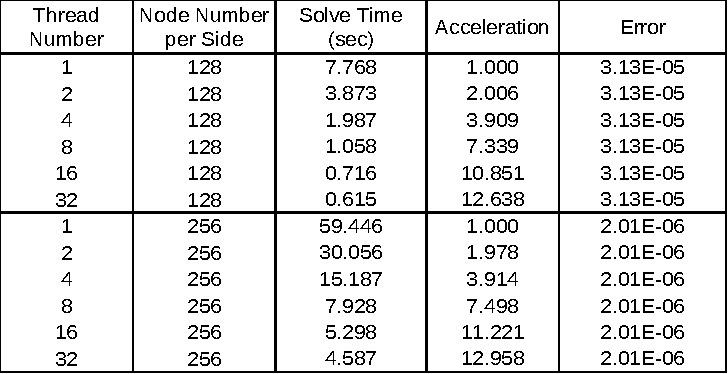
\includegraphics[width=\linewidth]{images/l1-omp.pdf}
     \caption{Зависимость времени решения от числа нитей процесса для $L = 1$}
     \label{tab:l1-omp}
   \end{minipage}\hfill
   \begin{minipage}{0.48\textwidth}
     \centering
     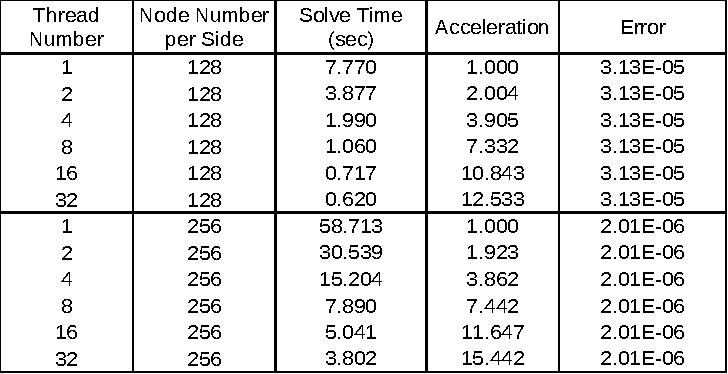
\includegraphics[width=\linewidth]{images/lp-omp.pdf}
     \caption{Зависимость времени решения от числа нитей процесса для $L = \pi$}
     \label{fig:lp-omp}
   \end{minipage}
\end{table}

\begin{figure}[h]
   \begin{minipage}{0.48\textwidth}
     \centering
     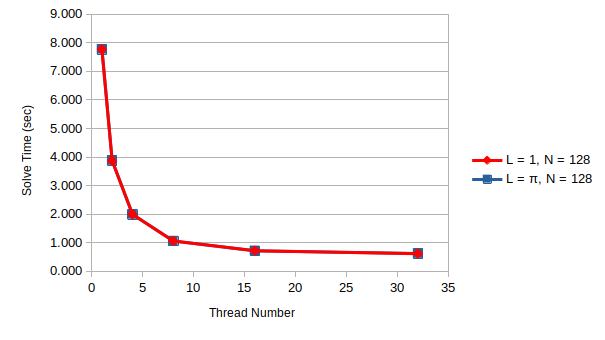
\includegraphics[width=\linewidth]{images/n128-omp.png}
     \caption{Зависимость времени решения от числа нитей процесса для $N = 128$}
     \label{fig:n128-omp}
   \end{minipage}\hfill
   \begin{minipage}{0.48\textwidth}
     \centering
     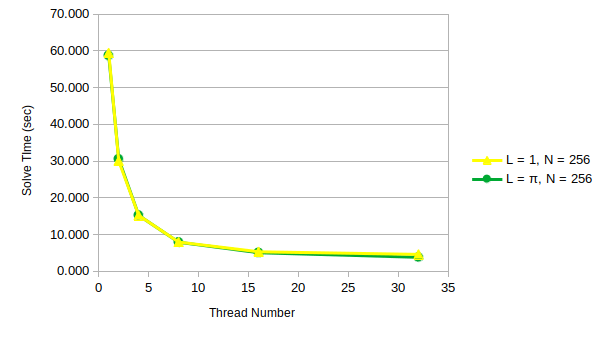
\includegraphics[width=\linewidth]{images/n256-omp.png}
     \caption{Зависимость времени решения от числа нитей процесса для $N = 256$}
     \label{fig:n256-omp}
   \end{minipage}
\end{figure}

\appendix

%\cleardoublepage \phantomsection
%\section*{Приложение}\label{sec:appendix}
%\addcontentsline{toc}{section}{Приложение}

\end{document}
